\newpage
\section{Zadanie 1}

\subsection{Opis zadania}

Dana jest funkcja
\[
Y = A \cdot B + C.
\]
Wyjście ma się załączyć, gdy jednocześnie są sygnały $A$ i $B$, albo gdy jest sam sygnał $C$. Jedno z tych dwóch wystarcza. $C$ nie pyta o $A$ ani o $B$, a iloczyn $A \cdot B$ nie pyta o $C$.

\subsection{Wejścia i wyjścia}

Trzy wejścia i jedna cewka. Przypisanie z programu jest w tabeli~\ref{tab:z1-io}.

\begin{table}[H]
    \centering
    \caption{Wejścia i wyjścia zadania 1}
    \label{tab:z1-io}
    \begin{tabular}{|l|l|p{8.2cm}|}
        \hline
        \textbf{Sygnał} & \textbf{Adres} & \textbf{Rola} \\
        \hline
        $A$ & I1 & pierwsze wejście iloczynu \\
        \hline
        $B$ & I2 & drugie wejście iloczynu \\
        \hline
        $C$ & I3 & osobna gałąź, sama załącza $Y$ \\
        \hline
        $Y$ & Q1 & wyjście \\
        \hline
    \end{tabular}
\end{table}

\subsection{Tablica prawdy}

Osiem kombinacji trzech wejść. Jedynka na $Y$ wypada tam, gdzie $C = 1$, oraz w jednym dodatkowym wierszu: $A = 1$, $B = 1$, $C = 0$.

\begin{table}[H]
    \centering
    \caption{Tablica prawdy funkcji $Y = A \cdot B + C$}
    \label{tab:z1-prawda}
    \begin{tabular}{|c|c|c|c|}
        \hline
        $A$ & $B$ & $C$ & $Y$ \\
        \hline
        0 & 0 & 0 & 0 \\
        \hline
        0 & 0 & 1 & 1 \\
        \hline
        0 & 1 & 0 & 0 \\
        \hline
        0 & 1 & 1 & 1 \\
        \hline
        1 & 0 & 0 & 0 \\
        \hline
        1 & 0 & 1 & 1 \\
        \hline
        1 & 1 & 0 & 1 \\
        \hline
        1 & 1 & 1 & 1 \\
        \hline
    \end{tabular}
\end{table}

\subsection{Funkcja logiczna}

Z pięciu wierszy, w których $Y = 1$, składamy sumę iloczynów. Zero na wejściu daje w iloczynie kreskę nad zmienną:

\begin{align*}
Y &= \overline{A}\,\overline{B}\,C + \overline{A}\,B\,C + A\,\overline{B}\,C \\
  &\quad + A\,B\,\overline{C} + A\,B\,C.
\end{align*}

To jest pełny zapis tablicy~\ref{tab:z1-prawda}, jeszcze przed sklejeniem.

\subsection{Minimalizacja}

Cztery iloczyny zawierające $C$ pokrywają wszystkie kombinacje $A$ i $B$:

\begin{align*}
\overline{A}\,\overline{B}\,C + \overline{A}\,B\,C + A\,\overline{B}\,C + A\,B\,C
  &= C\,(\overline{A}\,\overline{B} + \overline{A}\,B + A\,\overline{B} + A\,B) \\
  &= C.
\end{align*}

Zostaje $A\,B\,\overline{C}$. Skleja się z $A\,B\,C$, które już siedzi w $C$:

\[
A\,B\,\overline{C} + A\,B\,C = A\,B.
\]

Stąd
\[
Y = A \cdot B + C,
\]
czyli funkcja z polecenia. Krócej się tego nie zetnie. Samo $C$ gubi wiersz $A = 1$, $B = 1$, $C = 0$. Samo $A \cdot B$ gubi trzy wiersze, w których $C$ jest jedynką, a iloczyn $A \cdot B$ zerem.

\subsection{Schemat logiczny}

Po minimalizacji zostają dwie bramki. AND składa $A$ z $B$, OR dokłada do tego wyniku sygnał $C$. Wyjście bramki OR jest $Y$.

\begin{figure}[H]
    \centering
    \begin{circuitikz}[thick, font=\small]
        \node[and port] (ab) at (0,0.55) {};
        \node[or port] (wy) at (3.5,0) {};
        \draw (ab.in 1) -- ++(-1.05,0) node[left] {$A$};
        \draw (ab.in 2) -- ++(-1.05,0) node[left] {$B$};
        \draw (ab.out) -- ++(0.55,0) |- (wy.in 1);
        \draw (wy.in 2) -- ++(-1.15,0) node[left] {$C$};
        \draw (wy.out) -- ++(0.85,0) node[right] {$Y$};
    \end{circuitikz}
    \caption{Schemat logiczny $Y = A \cdot B + C$}
    \label{fig:z1-bramki}
\end{figure}

\subsection{Program PLC}

Na drabince z rys.~\ref{fig:z1-drabinka} górny szczebel ma I1 i I2 w szeregu. Dolny szczebel to sam I3. Obie gałęzie schodzą się w węźle przed cewką Q1. Szereg jest iloczynem, węzeł sumą, więc cewka dostaje $A \cdot B + C$.

\begin{figure}[H]
    \centering
    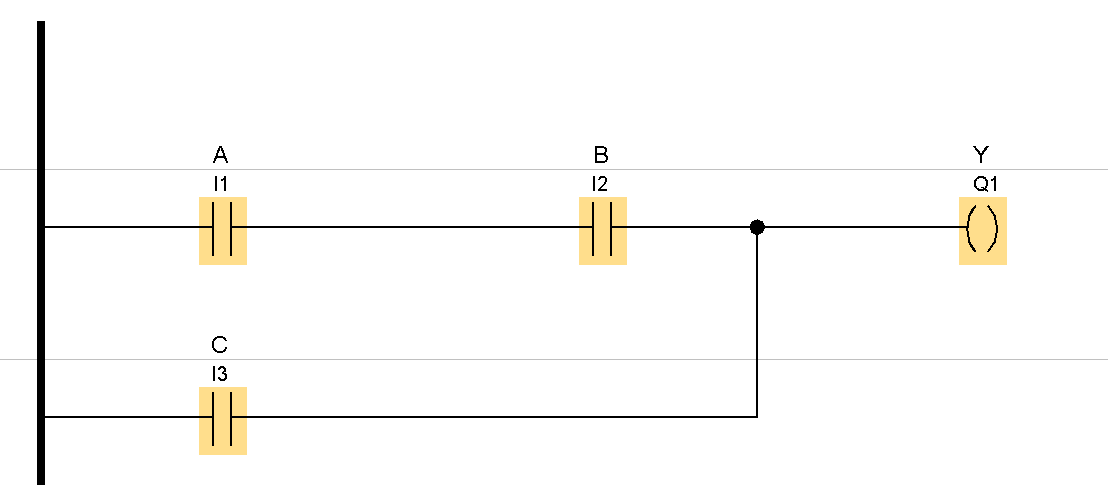
\includegraphics[width=0.82\textwidth]{rys/zad1/1_1_schemat.png}
    \caption{Drabinka zadania 1 w LOGO! Soft Comfort}
    \label{fig:z1-drabinka}
\end{figure}

W symulacji widać obie gałęzie z osobna. Przy $A = 1$, $B = 1$ i $C = 0$ świeci sam iloczyn (rys.~\ref{fig:z1-stany}a). Przy $A = 0$, $B = 0$ i $C = 1$ iloczyn jest zerem, a wyjście i tak wstaje, bo dolny szczebel nie patrzy na I1 ani I2 (rys.~\ref{fig:z1-stany}b). Trzeci stan dokłada do tego $B = 1$: iloczyn nadal jest zerem, skoro $A = 0$, a Q1 zostaje załączone przez $C$ (rys.~\ref{fig:z1-stany}c).

\begin{figure}[H]
    \centering
    \begin{subfigure}{\textwidth}
        \centering
        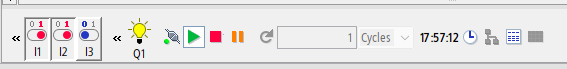
\includegraphics[width=0.70\textwidth]{rys/zad1/1_2_stan.png}
        \caption{$A = 1$, $B = 1$, $C = 0$, Q1 załączone}
    \end{subfigure}

    \vspace{0.4em}
    \begin{subfigure}{\textwidth}
        \centering
        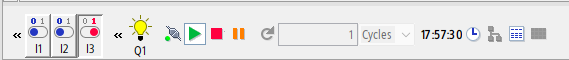
\includegraphics[width=0.70\textwidth]{rys/zad1/1_3_stan.png}
        \caption{$A = 0$, $B = 0$, $C = 1$, Q1 załączone}
    \end{subfigure}

    \vspace{0.4em}
    \begin{subfigure}{\textwidth}
        \centering
        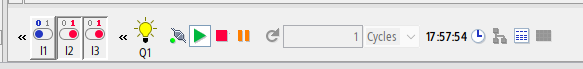
\includegraphics[width=0.70\textwidth]{rys/zad1/1_4stan.png}
        \caption{$A = 0$, $B = 1$, $C = 1$, Q1 załączone}
    \end{subfigure}
    \caption{Symulacja zadania 1. Czerwony przełącznik to jedynka, niebieski to zero}
    \label{fig:z1-stany}
\end{figure}
